\documentclass[1p]{elsarticle_modified}
%\bibliographystyle{elsarticle-num}

%\usepackage[colorlinks]{hyperref}
%\usepackage{abbrmath_seonhwa} %\Abb, \Ascr, \Acal ,\Abf, \Afrak
\usepackage{amsfonts}
\usepackage{amssymb}
\usepackage{amsmath}
\usepackage{amsthm}
\usepackage{scalefnt}
\usepackage{amsbsy}
\usepackage{kotex}
\usepackage{caption}
\usepackage{subfig}
\usepackage{color}
\usepackage{graphicx}
\usepackage{xcolor} %% white, black, red, green, blue, cyan, magenta, yellow
\usepackage{float}
\usepackage{setspace}
\usepackage{hyperref}

\usepackage{tikz}
\usetikzlibrary{arrows}

\usepackage{multirow}
\usepackage{array} % fixed length table
\usepackage{hhline}

%%%%%%%%%%%%%%%%%%%%%
\makeatletter
\renewcommand*\env@matrix[1][\arraystretch]{%
	\edef\arraystretch{#1}%
	\hskip -\arraycolsep
	\let\@ifnextchar\new@ifnextchar
	\array{*\c@MaxMatrixCols c}}
\makeatother %https://tex.stackexchange.com/questions/14071/how-can-i-increase-the-line-spacing-in-a-matrix
%%%%%%%%%%%%%%%

\usepackage[normalem]{ulem}

\newcommand{\msout}[1]{\ifmmode\text{\sout{\ensuremath{#1}}}\else\sout{#1}\fi}
%SOURCE: \msout is \stkout macro in https://tex.stackexchange.com/questions/20609/strikeout-in-math-mode

\newcommand{\cancel}[1]{
	\ifmmode
	{\color{red}\msout{#1}}
	\else
	{\color{red}\sout{#1}}
	\fi
}

\newcommand{\add}[1]{
	{\color{blue}\uwave{#1}}
}

\newcommand{\replace}[2]{
	\ifmmode
	{\color{red}\msout{#1}}{\color{blue}\uwave{#2}}
	\else
	{\color{red}\sout{#1}}{\color{blue}\uwave{#2}}
	\fi
}

\newcommand{\Sol}{\mathcal{S}} %segment
\newcommand{\D}{D} %diagram
\newcommand{\A}{\mathcal{A}} %arc


%%%%%%%%%%%%%%%%%%%%%%%%%%%%%5 test

\def\sl{\operatorname{\textup{SL}}(2,\Cbb)}
\def\psl{\operatorname{\textup{PSL}}(2,\Cbb)}
\def\quan{\mkern 1mu \triangleright \mkern 1mu}

\theoremstyle{definition}
\newtheorem{thm}{Theorem}[section]
\newtheorem{prop}[thm]{Proposition}
\newtheorem{lem}[thm]{Lemma}
\newtheorem{ques}[thm]{Question}
\newtheorem{cor}[thm]{Corollary}
\newtheorem{defn}[thm]{Definition}
\newtheorem{exam}[thm]{Example}
\newtheorem{rmk}[thm]{Remark}
\newtheorem{alg}[thm]{Algorithm}

\newcommand{\I}{\sqrt{-1}}
\begin{document}

%\begin{frontmatter}
%
%\title{Boundary parabolic representations of knots up to 8 crossings}
%
%%% Group authors per affiliation:
%\author{Yunhi Cho} 
%\address{Department of Mathematics, University of Seoul, Seoul, Korea}
%\ead{yhcho@uos.ac.kr}
%
%
%\author{Seonhwa Kim} %\fnref{s_kim}}
%\address{Center for Geometry and Physics, Institute for Basic Science, Pohang, 37673, Korea}
%\ead{ryeona17@ibs.re.kr}
%
%\author{Hyuk Kim}
%\address{Department of Mathematical Sciences, Seoul National University, Seoul 08826, Korea}
%\ead{hyukkim@snu.ac.kr}
%
%\author{Seokbeom Yoon}
%\address{Department of Mathematical Sciences, Seoul National University, Seoul, 08826,  Korea}
%\ead{sbyoon15@snu.ac.kr}
%
%\begin{abstract}
%We find all boundary parabolic representation of knots up to 8 crossings.
%
%\end{abstract}
%\begin{keyword}
%    \MSC[2010] 57M25 
%\end{keyword}
%
%\end{frontmatter}

%\linenumbers
%\tableofcontents
%
\newcommand\colored[1]{\textcolor{white}{\rule[-0.35ex]{0.8em}{1.4ex}}\kern-0.8em\color{red} #1}%
%\newcommand\colored[1]{\textcolor{white}{ #1}\kern-2.17ex	\textcolor{white}{ #1}\kern-1.81ex	\textcolor{white}{ #1}\kern-2.15ex\color{red}#1	}

{\Large $\underline{12a_{0786}~(K12a_{0786})}$}

\setlength{\tabcolsep}{10pt}
\renewcommand{\arraystretch}{1.6}
\vspace{1cm}\begin{tabular}{m{100pt}>{\centering\arraybackslash}m{274pt}}
\multirow{5}{120pt}{
	\centering
	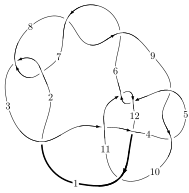
\includegraphics[width=112pt]{../../../GIT/diagram.site/Diagrams/png/1587_12a_0786.png}\\
\ \ \ A knot diagram\footnotemark}&
\allowdisplaybreaks
\textbf{Linearized knot diagam} \\
\cline{2-2}
 &
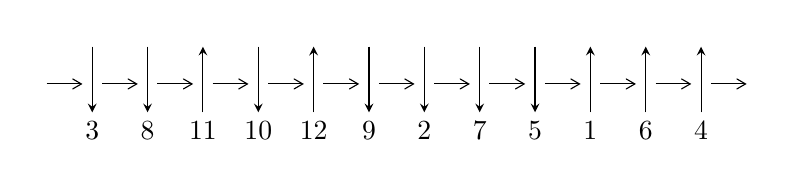
\begin{tikzpicture}[x=20pt, y=17pt]
	% nodes
	\node (C0) at (0, 0) {};
	\node (C1) at (1, 0) {};
	\node (C1U) at (1, +1) {};
	\node (C1D) at (1, -1) {3};

	\node (C2) at (2, 0) {};
	\node (C2U) at (2, +1) {};
	\node (C2D) at (2, -1) {8};

	\node (C3) at (3, 0) {};
	\node (C3U) at (3, +1) {};
	\node (C3D) at (3, -1) {11};

	\node (C4) at (4, 0) {};
	\node (C4U) at (4, +1) {};
	\node (C4D) at (4, -1) {10};

	\node (C5) at (5, 0) {};
	\node (C5U) at (5, +1) {};
	\node (C5D) at (5, -1) {12};

	\node (C6) at (6, 0) {};
	\node (C6U) at (6, +1) {};
	\node (C6D) at (6, -1) {9};

	\node (C7) at (7, 0) {};
	\node (C7U) at (7, +1) {};
	\node (C7D) at (7, -1) {2};

	\node (C8) at (8, 0) {};
	\node (C8U) at (8, +1) {};
	\node (C8D) at (8, -1) {7};

	\node (C9) at (9, 0) {};
	\node (C9U) at (9, +1) {};
	\node (C9D) at (9, -1) {5};

	\node (C10) at (10, 0) {};
	\node (C10U) at (10, +1) {};
	\node (C10D) at (10, -1) {1};

	\node (C11) at (11, 0) {};
	\node (C11U) at (11, +1) {};
	\node (C11D) at (11, -1) {6};

	\node (C12) at (12, 0) {};
	\node (C12U) at (12, +1) {};
	\node (C12D) at (12, -1) {4};
	\node (C13) at (13, 0) {};

	% arrows
	\draw[->,>={angle 60}]
	(C0) edge (C1) (C1) edge (C2) (C2) edge (C3) (C3) edge (C4) (C4) edge (C5) (C5) edge (C6) (C6) edge (C7) (C7) edge (C8) (C8) edge (C9) (C9) edge (C10) (C10) edge (C11) (C11) edge (C12) (C12) edge (C13) ;	\draw[->,>=stealth]
	(C1U) edge (C1D) (C2U) edge (C2D) (C3D) edge (C3U) (C4U) edge (C4D) (C5D) edge (C5U) (C6U) edge (C6D) (C7U) edge (C7D) (C8U) edge (C8D) (C9U) edge (C9D) (C10D) edge (C10U) (C11D) edge (C11U) (C12D) edge (C12U) ;
	\end{tikzpicture} \\
\hhline{~~} \\& 
\textbf{Solving Sequence} \\ \cline{2-2} 
 &
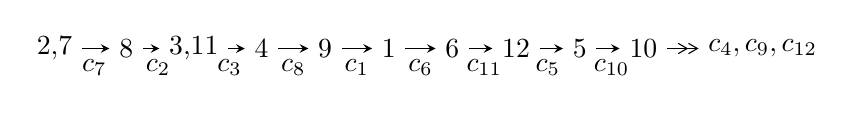
\begin{tikzpicture}[x=23pt, y=7pt]
	% node
	\node (A0) at (-1/8, 0) {2,7};
	\node (A1) at (1, 0) {8};
	\node (A2) at (33/16, 0) {3,11};
	\node (A3) at (25/8, 0) {4};
	\node (A4) at (33/8, 0) {9};
	\node (A5) at (41/8, 0) {1};
	\node (A6) at (49/8, 0) {6};
	\node (A7) at (57/8, 0) {12};
	\node (A8) at (65/8, 0) {5};
	\node (A9) at (73/8, 0) {10};
	\node (C1) at (1/2, -1) {$c_{7}$};
	\node (C2) at (3/2, -1) {$c_{2}$};
	\node (C3) at (21/8, -1) {$c_{3}$};
	\node (C4) at (29/8, -1) {$c_{8}$};
	\node (C5) at (37/8, -1) {$c_{1}$};
	\node (C6) at (45/8, -1) {$c_{6}$};
	\node (C7) at (53/8, -1) {$c_{11}$};
	\node (C8) at (61/8, -1) {$c_{5}$};
	\node (C9) at (69/8, -1) {$c_{10}$};
	\node (A10) at (11, 0) {$c_{4},c_{9},c_{12}$};

	% edge
	\draw[->,>=stealth]	
	(A0) edge (A1) (A1) edge (A2) (A2) edge (A3) (A3) edge (A4) (A4) edge (A5) (A5) edge (A6) (A6) edge (A7) (A7) edge (A8) (A8) edge (A9) ;
	\draw[->>,>={angle 60}]	
	(A9) edge (A10);
\end{tikzpicture} \\ 

\end{tabular} \\

\footnotetext{
The image of knot diagram is generated by the software ``\textbf{Draw programme}" developed by Andrew Bartholomew(\url{http://www.layer8.co.uk/maths/draw/index.htm\#Running-draw}), where we modified some parts for our purpose(\url{https://github.com/CATsTAILs/LinksPainter}).
}\phantom \\ \newline 
\centering \textbf{Ideals for irreducible components\footnotemark of $X_{\text{par}}$} 
 
\begin{align*}
I^u_{1}&=\langle 
7.76879\times10^{80} u^{103}+8.52236\times10^{80} u^{102}+\cdots+3.56472\times10^{80} b-4.99373\times10^{81},\\
\phantom{I^u_{1}}&\phantom{= \langle  }-6.43118\times10^{80} u^{103}-4.09372\times10^{81} u^{102}+\cdots+2.49530\times10^{81} a+1.23254\times10^{82},\;u^{104}+u^{103}+\cdots-7 u+7\rangle \\
I^u_{2}&=\langle 
-2 u^{19}+5 u^{17}+\cdots+b-1,\;2 u^{19}- u^{18}+\cdots+a-1,\;u^{20}-3 u^{18}+\cdots+u+1\rangle \\
\\
\end{align*}
\raggedright * 2 irreducible components of $\dim_{\mathbb{C}}=0$, with total 124 representations.\\
\footnotetext{All coefficients of polynomials are rational numbers. But the coefficients are sometimes approximated in decimal forms when there is not enough margin.}
\newpage
\renewcommand{\arraystretch}{1}
\centering \section*{I. $I^u_{1}= \langle 7.77\times10^{80} u^{103}+8.52\times10^{80} u^{102}+\cdots+3.56\times10^{80} b-4.99\times10^{81},\;-6.43\times10^{80} u^{103}-4.09\times10^{81} u^{102}+\cdots+2.50\times10^{81} a+1.23\times10^{82},\;u^{104}+u^{103}+\cdots-7 u+7 \rangle$}
\flushleft \textbf{(i) Arc colorings}\\
\begin{tabular}{m{7pt} m{180pt} m{7pt} m{180pt} }
\flushright $a_{2}=$&$\begin{pmatrix}0\\u\end{pmatrix}$ \\
\flushright $a_{7}=$&$\begin{pmatrix}1\\0\end{pmatrix}$ \\
\flushright $a_{8}=$&$\begin{pmatrix}1\\u^2\end{pmatrix}$ \\
\flushright $a_{3}=$&$\begin{pmatrix}- u\\- u^3+u\end{pmatrix}$ \\
\flushright $a_{11}=$&$\begin{pmatrix}0.257732 u^{103}+1.64057 u^{102}+\cdots-20.8766 u-4.93944\\-2.17936 u^{103}-2.39075 u^{102}+\cdots+25.2220 u+14.0088\end{pmatrix}$ \\
\flushright $a_{4}=$&$\begin{pmatrix}4.54650 u^{103}+4.71983 u^{102}+\cdots-21.6024 u-22.5070\\0.732669 u^{103}+0.154268 u^{102}+\cdots+7.64667 u+3.76015\end{pmatrix}$ \\
\flushright $a_{9}=$&$\begin{pmatrix}- u^2+1\\u^2\end{pmatrix}$ \\
\flushright $a_{1}=$&$\begin{pmatrix}u^3\\u^5- u^3+u\end{pmatrix}$ \\
\flushright $a_{6}=$&$\begin{pmatrix}u^4- u^2+1\\- u^4\end{pmatrix}$ \\
\flushright $a_{12}=$&$\begin{pmatrix}-1.07483 u^{103}+0.848416 u^{102}+\cdots-4.82910 u-1.91321\\-2.87953 u^{103}-3.09296 u^{102}+\cdots+28.4903 u+13.0462\end{pmatrix}$ \\
\flushright $a_{5}=$&$\begin{pmatrix}1.07670 u^{103}+1.40144 u^{102}+\cdots+0.0336515 u-10.1638\\-0.478154 u^{103}-0.659756 u^{102}+\cdots+20.1108 u+3.76858\end{pmatrix}$ \\
\flushright $a_{10}=$&$\begin{pmatrix}-0.224309 u^{103}+2.43305 u^{102}+\cdots-12.2602 u-13.0672\\-1.89620 u^{103}-2.01139 u^{102}+\cdots+26.0423 u+7.99311\end{pmatrix}$\\&\end{tabular}
\flushleft \textbf{(ii) Obstruction class $= -1$}\\~\\
\flushleft \textbf{(iii) Cusp Shapes $= 4.36792 u^{103}+16.1678 u^{102}+\cdots-14.8053 u-125.030$}\\~\\
\newpage\renewcommand{\arraystretch}{1}
\flushleft \textbf{(iv) u-Polynomials at the component}\newline \\
\begin{tabular}{m{50pt}|m{274pt}}
Crossings & \hspace{64pt}u-Polynomials at each crossing \\
\hline $$\begin{aligned}c_{1},c_{6},c_{8}\end{aligned}$$&$\begin{aligned}
&u^{104}+25 u^{103}+\cdots+749 u+49
\end{aligned}$\\
\hline $$\begin{aligned}c_{2},c_{7}\end{aligned}$$&$\begin{aligned}
&u^{104}+u^{103}+\cdots-7 u+7
\end{aligned}$\\
\hline $$\begin{aligned}c_{3}\end{aligned}$$&$\begin{aligned}
&u^{104}-10 u^{102}+\cdots+34258 u+3709
\end{aligned}$\\
\hline $$\begin{aligned}c_{4},c_{9}\end{aligned}$$&$\begin{aligned}
&u^{104}-2 u^{103}+\cdots-728 u+121
\end{aligned}$\\
\hline $$\begin{aligned}c_{5},c_{11}\end{aligned}$$&$\begin{aligned}
&u^{104}- u^{103}+\cdots- u+7
\end{aligned}$\\
\hline $$\begin{aligned}c_{10}\end{aligned}$$&$\begin{aligned}
&u^{104}+11 u^{103}+\cdots+131198 u+14113
\end{aligned}$\\
\hline $$\begin{aligned}c_{12}\end{aligned}$$&$\begin{aligned}
&u^{104}+7 u^{103}+\cdots- u+1
\end{aligned}$\\
\hline
\end{tabular}\\~\\
\newpage\renewcommand{\arraystretch}{1}
\flushleft \textbf{(v) Riley Polynomials at the component}\newline \\
\begin{tabular}{m{50pt}|m{274pt}}
Crossings & \hspace{64pt}Riley Polynomials at each crossing \\
\hline $$\begin{aligned}c_{1},c_{6},c_{8}\end{aligned}$$&$\begin{aligned}
&y^{104}+115 y^{103}+\cdots+32487 y+2401
\end{aligned}$\\
\hline $$\begin{aligned}c_{2},c_{7}\end{aligned}$$&$\begin{aligned}
&y^{104}-25 y^{103}+\cdots-749 y+49
\end{aligned}$\\
\hline $$\begin{aligned}c_{3}\end{aligned}$$&$\begin{aligned}
&y^{104}-20 y^{103}+\cdots-305407844 y+13756681
\end{aligned}$\\
\hline $$\begin{aligned}c_{4},c_{9}\end{aligned}$$&$\begin{aligned}
&y^{104}+76 y^{103}+\cdots+509890 y+14641
\end{aligned}$\\
\hline $$\begin{aligned}c_{5},c_{11}\end{aligned}$$&$\begin{aligned}
&y^{104}+57 y^{103}+\cdots+1693 y+49
\end{aligned}$\\
\hline $$\begin{aligned}c_{10}\end{aligned}$$&$\begin{aligned}
&y^{104}-43 y^{103}+\cdots-10011615824 y+199176769
\end{aligned}$\\
\hline $$\begin{aligned}c_{12}\end{aligned}$$&$\begin{aligned}
&y^{104}-5 y^{103}+\cdots+89 y+1
\end{aligned}$\\
\hline
\end{tabular}\\~\\
\newpage\flushleft \textbf{(vi) Complex Volumes and Cusp Shapes}
$$\begin{array}{c|c|c}  
\text{Solutions to }I^u_{1}& \I (\text{vol} + \sqrt{-1}CS) & \text{Cusp shape}\\
 \hline 
\begin{aligned}
u &= \phantom{-}0.766662 + 0.632934 I \\
a &= \phantom{-}0.157630 + 0.376131 I \\
b &= \phantom{-}0.354923 + 0.313305 I\end{aligned}
 & \phantom{-}2.70022 - 2.40792 I & \phantom{-0.000000 } 0 \\ \hline\begin{aligned}
u &= \phantom{-}0.766662 - 0.632934 I \\
a &= \phantom{-}0.157630 - 0.376131 I \\
b &= \phantom{-}0.354923 - 0.313305 I\end{aligned}
 & \phantom{-}2.70022 + 2.40792 I & \phantom{-0.000000 } 0 \\ \hline\begin{aligned}
u &= \phantom{-}0.990161 + 0.226156 I \\
a &= \phantom{-}0.345510 + 0.630720 I \\
b &= \phantom{-}0.456131 - 0.442211 I\end{aligned}
 & -0.06685 - 3.01354 I & \phantom{-0.000000 } 0 \\ \hline\begin{aligned}
u &= \phantom{-}0.990161 - 0.226156 I \\
a &= \phantom{-}0.345510 - 0.630720 I \\
b &= \phantom{-}0.456131 + 0.442211 I\end{aligned}
 & -0.06685 + 3.01354 I & \phantom{-0.000000 } 0 \\ \hline\begin{aligned}
u &= -0.898218 + 0.484385 I \\
a &= -0.375200 + 1.107920 I \\
b &= \phantom{-}0.789176 - 1.165220 I\end{aligned}
 & \phantom{-}3.58702 + 6.98929 I & \phantom{-0.000000 } 0 \\ \hline\begin{aligned}
u &= -0.898218 - 0.484385 I \\
a &= -0.375200 - 1.107920 I \\
b &= \phantom{-}0.789176 + 1.165220 I\end{aligned}
 & \phantom{-}3.58702 - 6.98929 I & \phantom{-0.000000 } 0 \\ \hline\begin{aligned}
u &= \phantom{-}0.906841 + 0.328078 I \\
a &= \phantom{-}1.43990 + 0.82818 I \\
b &= -0.805047 - 0.092018 I\end{aligned}
 & -1.74282 - 5.46943 I & \phantom{-0.000000 } 0 \\ \hline\begin{aligned}
u &= \phantom{-}0.906841 - 0.328078 I \\
a &= \phantom{-}1.43990 - 0.82818 I \\
b &= -0.805047 + 0.092018 I\end{aligned}
 & -1.74282 + 5.46943 I & \phantom{-0.000000 } 0 \\ \hline\begin{aligned}
u &= \phantom{-}0.731510 + 0.614247 I \\
a &= -0.229128 + 0.377392 I \\
b &= \phantom{-}0.452360 + 0.444639 I\end{aligned}
 & \phantom{-}2.77148 - 2.27111 I & \phantom{-0.000000 } 0 \\ \hline\begin{aligned}
u &= \phantom{-}0.731510 - 0.614247 I \\
a &= -0.229128 - 0.377392 I \\
b &= \phantom{-}0.452360 - 0.444639 I\end{aligned}
 & \phantom{-}2.77148 + 2.27111 I & \phantom{-0.000000 } 0\\
 \hline 
 \end{array}$$\newpage$$\begin{array}{c|c|c}  
\text{Solutions to }I^u_{1}& \I (\text{vol} + \sqrt{-1}CS) & \text{Cusp shape}\\
 \hline 
\begin{aligned}
u &= -0.946665 + 0.445873 I \\
a &= \phantom{-}1.110950 - 0.256330 I \\
b &= -0.172865 + 0.593087 I\end{aligned}
 & -3.47387 + 7.06916 I & \phantom{-0.000000 } 0 \\ \hline\begin{aligned}
u &= -0.946665 - 0.445873 I \\
a &= \phantom{-}1.110950 + 0.256330 I \\
b &= -0.172865 - 0.593087 I\end{aligned}
 & -3.47387 - 7.06916 I & \phantom{-0.000000 } 0 \\ \hline\begin{aligned}
u &= \phantom{-}0.429102 + 0.835909 I \\
a &= \phantom{-}0.621121 - 0.556923 I \\
b &= -0.449537 + 0.417666 I\end{aligned}
 & \phantom{-}3.48038 - 4.88988 I & \phantom{-0.000000 } 0 \\ \hline\begin{aligned}
u &= \phantom{-}0.429102 - 0.835909 I \\
a &= \phantom{-}0.621121 + 0.556923 I \\
b &= -0.449537 - 0.417666 I\end{aligned}
 & \phantom{-}3.48038 + 4.88988 I & \phantom{-0.000000 } 0 \\ \hline\begin{aligned}
u &= \phantom{-}0.933574 + 0.046772 I \\
a &= \phantom{-}0.268196 - 0.407068 I \\
b &= -0.577101 - 1.046790 I\end{aligned}
 & -5.72348 + 1.88899 I & \phantom{-0.000000 } 0 \\ \hline\begin{aligned}
u &= \phantom{-}0.933574 - 0.046772 I \\
a &= \phantom{-}0.268196 + 0.407068 I \\
b &= -0.577101 + 1.046790 I\end{aligned}
 & -5.72348 - 1.88899 I & \phantom{-0.000000 } 0 \\ \hline\begin{aligned}
u &= \phantom{-}0.855864 + 0.353216 I \\
a &= \phantom{-}0.512007 + 0.795136 I \\
b &= -0.105151 - 0.893329 I\end{aligned}
 & -0.24953 - 3.56298 I & \phantom{-0.000000 } 0 \\ \hline\begin{aligned}
u &= \phantom{-}0.855864 - 0.353216 I \\
a &= \phantom{-}0.512007 - 0.795136 I \\
b &= -0.105151 + 0.893329 I\end{aligned}
 & -0.24953 + 3.56298 I & \phantom{-0.000000 } 0 \\ \hline\begin{aligned}
u &= -0.901014 + 0.209728 I \\
a &= -0.667920 - 0.366820 I \\
b &= -0.404203 + 1.238470 I\end{aligned}
 & -2.37554 - 0.53656 I & \phantom{-0.000000 } 0 \\ \hline\begin{aligned}
u &= -0.901014 - 0.209728 I \\
a &= -0.667920 + 0.366820 I \\
b &= -0.404203 - 1.238470 I\end{aligned}
 & -2.37554 + 0.53656 I & \phantom{-0.000000 } 0\\
 \hline 
 \end{array}$$\newpage$$\begin{array}{c|c|c}  
\text{Solutions to }I^u_{1}& \I (\text{vol} + \sqrt{-1}CS) & \text{Cusp shape}\\
 \hline 
\begin{aligned}
u &= -0.872757 + 0.636215 I \\
a &= -0.921173 - 0.839949 I \\
b &= \phantom{-}0.145920 + 0.925194 I\end{aligned}
 & -2.23261 + 2.46085 I & \phantom{-0.000000 } 0 \\ \hline\begin{aligned}
u &= -0.872757 - 0.636215 I \\
a &= -0.921173 + 0.839949 I \\
b &= \phantom{-}0.145920 - 0.925194 I\end{aligned}
 & -2.23261 - 2.46085 I & \phantom{-0.000000 } 0 \\ \hline\begin{aligned}
u &= -1.081480 + 0.026581 I \\
a &= -0.133652 - 0.172093 I \\
b &= \phantom{-}0.616078 - 0.692280 I\end{aligned}
 & -2.16276 - 6.51848 I & \phantom{-0.000000 } 0 \\ \hline\begin{aligned}
u &= -1.081480 - 0.026581 I \\
a &= -0.133652 + 0.172093 I \\
b &= \phantom{-}0.616078 + 0.692280 I\end{aligned}
 & -2.16276 + 6.51848 I & \phantom{-0.000000 } 0 \\ \hline\begin{aligned}
u &= -0.795173 + 0.379218 I \\
a &= -1.78364 - 0.31075 I \\
b &= \phantom{-}0.736381 + 0.569274 I\end{aligned}
 & -2.74142 + 1.90360 I & \phantom{-0.000000 } 0 \\ \hline\begin{aligned}
u &= -0.795173 - 0.379218 I \\
a &= -1.78364 + 0.31075 I \\
b &= \phantom{-}0.736381 - 0.569274 I\end{aligned}
 & -2.74142 - 1.90360 I & \phantom{-0.000000 } 0 \\ \hline\begin{aligned}
u &= -0.780756 + 0.394948 I \\
a &= \phantom{-}1.63110 - 0.64652 I \\
b &= \phantom{-}0.735324 - 0.701901 I\end{aligned}
 & \phantom{-}1.33892 + 4.93257 I & \phantom{-0.000000 } 0 \\ \hline\begin{aligned}
u &= -0.780756 - 0.394948 I \\
a &= \phantom{-}1.63110 + 0.64652 I \\
b &= \phantom{-}0.735324 + 0.701901 I\end{aligned}
 & \phantom{-}1.33892 - 4.93257 I & \phantom{-0.000000 } 0 \\ \hline\begin{aligned}
u &= -1.064430 + 0.374375 I \\
a &= -0.296034 + 0.425423 I \\
b &= -0.436153 - 0.006085 I\end{aligned}
 & \phantom{-}0.83535 + 3.47388 I & \phantom{-0.000000 } 0 \\ \hline\begin{aligned}
u &= -1.064430 - 0.374375 I \\
a &= -0.296034 - 0.425423 I \\
b &= -0.436153 + 0.006085 I\end{aligned}
 & \phantom{-}0.83535 - 3.47388 I & \phantom{-0.000000 } 0\\
 \hline 
 \end{array}$$\newpage$$\begin{array}{c|c|c}  
\text{Solutions to }I^u_{1}& \I (\text{vol} + \sqrt{-1}CS) & \text{Cusp shape}\\
 \hline 
\begin{aligned}
u &= \phantom{-}1.032620 + 0.455050 I \\
a &= -0.868126 - 0.506848 I \\
b &= \phantom{-}0.136396 + 0.458095 I\end{aligned}
 & \phantom{-}0.43075 - 13.03650 I & \phantom{-0.000000 } 0 \\ \hline\begin{aligned}
u &= \phantom{-}1.032620 - 0.455050 I \\
a &= -0.868126 + 0.506848 I \\
b &= \phantom{-}0.136396 - 0.458095 I\end{aligned}
 & \phantom{-}0.43075 + 13.03650 I & \phantom{-0.000000 } 0 \\ \hline\begin{aligned}
u &= \phantom{-}0.300979 + 0.788432 I \\
a &= \phantom{-}0.941826 + 0.087842 I \\
b &= -0.158311 - 0.511357 I\end{aligned}
 & \phantom{-}2.84217 + 8.57300 I & \phantom{-0.000000 } 0 \\ \hline\begin{aligned}
u &= \phantom{-}0.300979 - 0.788432 I \\
a &= \phantom{-}0.941826 - 0.087842 I \\
b &= -0.158311 + 0.511357 I\end{aligned}
 & \phantom{-}2.84217 - 8.57300 I & \phantom{-0.000000 } 0 \\ \hline\begin{aligned}
u &= \phantom{-}0.895050 + 0.778119 I \\
a &= -0.0114617 + 0.1300560 I \\
b &= \phantom{-}0.458745 + 0.554629 I\end{aligned}
 & \phantom{-}3.11399 - 2.93489 I & \phantom{-0.000000 } 0 \\ \hline\begin{aligned}
u &= \phantom{-}0.895050 - 0.778119 I \\
a &= -0.0114617 - 0.1300560 I \\
b &= \phantom{-}0.458745 - 0.554629 I\end{aligned}
 & \phantom{-}3.11399 + 2.93489 I & \phantom{-0.000000 } 0 \\ \hline\begin{aligned}
u &= -0.468867 + 0.652301 I \\
a &= \phantom{-}1.67663 - 0.15872 I \\
b &= -0.769802 - 0.269370 I\end{aligned}
 & \phantom{-}4.96708 - 2.78599 I & \phantom{-}5.45184 + 0. I\phantom{ +0.000000I} \\ \hline\begin{aligned}
u &= -0.468867 - 0.652301 I \\
a &= \phantom{-}1.67663 + 0.15872 I \\
b &= -0.769802 + 0.269370 I\end{aligned}
 & \phantom{-}4.96708 + 2.78599 I & \phantom{-}5.45184 + 0. I\phantom{ +0.000000I} \\ \hline\begin{aligned}
u &= -0.837269 + 0.858305 I \\
a &= \phantom{-}1.71955 - 1.12101 I \\
b &= -2.47926 - 0.90809 I\end{aligned}
 & \phantom{-}6.98765 - 0.83385 I & \phantom{-0.000000 } 0 \\ \hline\begin{aligned}
u &= -0.837269 - 0.858305 I \\
a &= \phantom{-}1.71955 + 1.12101 I \\
b &= -2.47926 + 0.90809 I\end{aligned}
 & \phantom{-}6.98765 + 0.83385 I & \phantom{-0.000000 } 0\\
 \hline 
 \end{array}$$\newpage$$\begin{array}{c|c|c}  
\text{Solutions to }I^u_{1}& \I (\text{vol} + \sqrt{-1}CS) & \text{Cusp shape}\\
 \hline 
\begin{aligned}
u &= -0.857688 + 0.848054 I \\
a &= \phantom{-}1.34507 - 1.62875 I \\
b &= -3.28470 - 0.20003 I\end{aligned}
 & \phantom{-}5.55138 - 2.69728 I & \phantom{-0.000000 } 0 \\ \hline\begin{aligned}
u &= -0.857688 - 0.848054 I \\
a &= \phantom{-}1.34507 + 1.62875 I \\
b &= -3.28470 + 0.20003 I\end{aligned}
 & \phantom{-}5.55138 + 2.69728 I & \phantom{-0.000000 } 0 \\ \hline\begin{aligned}
u &= \phantom{-}0.727404 + 0.308828 I \\
a &= \phantom{-}1.55109 - 0.19015 I \\
b &= -0.07706 + 1.94742 I\end{aligned}
 & -3.22727 - 1.25096 I & -2.00000 + 7.02823 I \\ \hline\begin{aligned}
u &= \phantom{-}0.727404 - 0.308828 I \\
a &= \phantom{-}1.55109 + 0.19015 I \\
b &= -0.07706 - 1.94742 I\end{aligned}
 & -3.22727 + 1.25096 I & -2.00000 - 7.02823 I \\ \hline\begin{aligned}
u &= \phantom{-}1.078300 + 0.561549 I \\
a &= \phantom{-}0.288763 - 0.501283 I \\
b &= \phantom{-}0.140095 + 0.441770 I\end{aligned}
 & \phantom{-}1.39183 - 0.25582 I & \phantom{-0.000000 } 0 \\ \hline\begin{aligned}
u &= \phantom{-}1.078300 - 0.561549 I \\
a &= \phantom{-}0.288763 + 0.501283 I \\
b &= \phantom{-}0.140095 - 0.441770 I\end{aligned}
 & \phantom{-}1.39183 + 0.25582 I & \phantom{-0.000000 } 0 \\ \hline\begin{aligned}
u &= -0.757240 + 0.174967 I \\
a &= \phantom{-}0.039857 - 0.279716 I \\
b &= -0.536813 + 0.538199 I\end{aligned}
 & -1.263330 + 0.418486 I & -7.09557 - 0.72347 I \\ \hline\begin{aligned}
u &= -0.757240 - 0.174967 I \\
a &= \phantom{-}0.039857 + 0.279716 I \\
b &= -0.536813 - 0.538199 I\end{aligned}
 & -1.263330 - 0.418486 I & -7.09557 + 0.72347 I \\ \hline\begin{aligned}
u &= -0.890714 + 0.843520 I \\
a &= \phantom{-}1.90421 - 1.78407 I \\
b &= -3.15861 - 0.74730 I\end{aligned}
 & \phantom{-}6.78735 - 0.08301 I & \phantom{-0.000000 } 0 \\ \hline\begin{aligned}
u &= -0.890714 - 0.843520 I \\
a &= \phantom{-}1.90421 + 1.78407 I \\
b &= -3.15861 + 0.74730 I\end{aligned}
 & \phantom{-}6.78735 + 0.08301 I & \phantom{-0.000000 } 0\\
 \hline 
 \end{array}$$\newpage$$\begin{array}{c|c|c}  
\text{Solutions to }I^u_{1}& \I (\text{vol} + \sqrt{-1}CS) & \text{Cusp shape}\\
 \hline 
\begin{aligned}
u &= \phantom{-}0.890419 + 0.847639 I \\
a &= -0.66583 - 1.29156 I \\
b &= \phantom{-}2.37783 + 0.54118 I\end{aligned}
 & \phantom{-}4.51852 - 1.93015 I & \phantom{-0.000000 } 0 \\ \hline\begin{aligned}
u &= \phantom{-}0.890419 - 0.847639 I \\
a &= -0.66583 + 1.29156 I \\
b &= \phantom{-}2.37783 - 0.54118 I\end{aligned}
 & \phantom{-}4.51852 + 1.93015 I & \phantom{-0.000000 } 0 \\ \hline\begin{aligned}
u &= \phantom{-}0.818432 + 0.920455 I \\
a &= -1.46291 - 0.80542 I \\
b &= \phantom{-}2.13933 - 0.57457 I\end{aligned}
 & \phantom{-}9.65675 + 2.00371 I & \phantom{-0.000000 } 0 \\ \hline\begin{aligned}
u &= \phantom{-}0.818432 - 0.920455 I \\
a &= -1.46291 + 0.80542 I \\
b &= \phantom{-}2.13933 + 0.57457 I\end{aligned}
 & \phantom{-}9.65675 - 2.00371 I & \phantom{-0.000000 } 0 \\ \hline\begin{aligned}
u &= \phantom{-}0.717756 + 0.257429 I \\
a &= -2.47456 - 0.58230 I \\
b &= -0.198074 + 0.179300 I\end{aligned}
 & \phantom{-}0.59876 + 1.75726 I & -4.14188 + 1.37130 I \\ \hline\begin{aligned}
u &= \phantom{-}0.717756 - 0.257429 I \\
a &= -2.47456 + 0.58230 I \\
b &= -0.198074 - 0.179300 I\end{aligned}
 & \phantom{-}0.59876 - 1.75726 I & -4.14188 - 1.37130 I \\ \hline\begin{aligned}
u &= -0.908019 + 0.843254 I \\
a &= \phantom{-}0.037172 + 0.239025 I \\
b &= -0.474318 + 0.556665 I\end{aligned}
 & \phantom{-}3.46367 + 3.13699 I & \phantom{-0.000000 } 0 \\ \hline\begin{aligned}
u &= -0.908019 - 0.843254 I \\
a &= \phantom{-}0.037172 - 0.239025 I \\
b &= -0.474318 - 0.556665 I\end{aligned}
 & \phantom{-}3.46367 - 3.13699 I & \phantom{-0.000000 } 0 \\ \hline\begin{aligned}
u &= -0.922624 + 0.832948 I \\
a &= -1.81548 + 1.58635 I \\
b &= \phantom{-}3.50548 + 0.24041 I\end{aligned}
 & \phantom{-}6.68785 + 6.32651 I & \phantom{-0.000000 } 0 \\ \hline\begin{aligned}
u &= -0.922624 - 0.832948 I \\
a &= -1.81548 - 1.58635 I \\
b &= \phantom{-}3.50548 - 0.24041 I\end{aligned}
 & \phantom{-}6.68785 - 6.32651 I & \phantom{-0.000000 } 0\\
 \hline 
 \end{array}$$\newpage$$\begin{array}{c|c|c}  
\text{Solutions to }I^u_{1}& \I (\text{vol} + \sqrt{-1}CS) & \text{Cusp shape}\\
 \hline 
\begin{aligned}
u &= \phantom{-}0.860422 + 0.899570 I \\
a &= \phantom{-}1.18975 + 2.21934 I \\
b &= -3.18431 - 0.74729 I\end{aligned}
 & \phantom{-}5.25028 + 4.20090 I & \phantom{-0.000000 } 0 \\ \hline\begin{aligned}
u &= \phantom{-}0.860422 - 0.899570 I \\
a &= \phantom{-}1.18975 - 2.21934 I \\
b &= -3.18431 + 0.74729 I\end{aligned}
 & \phantom{-}5.25028 - 4.20090 I & \phantom{-0.000000 } 0 \\ \hline\begin{aligned}
u &= -0.835559 + 0.923554 I \\
a &= -1.35608 + 1.79331 I \\
b &= \phantom{-}2.93378 - 0.19568 I\end{aligned}
 & \phantom{-}9.6493 - 11.0115 I & \phantom{-0.000000 } 0 \\ \hline\begin{aligned}
u &= -0.835559 - 0.923554 I \\
a &= -1.35608 - 1.79331 I \\
b &= \phantom{-}2.93378 + 0.19568 I\end{aligned}
 & \phantom{-}9.6493 + 11.0115 I & \phantom{-0.000000 } 0 \\ \hline\begin{aligned}
u &= \phantom{-}0.897180 + 0.864300 I \\
a &= \phantom{-}2.40675 + 0.58401 I \\
b &= -3.07009 + 1.40635 I\end{aligned}
 & \phantom{-}8.90543 + 0.76441 I & \phantom{-0.000000 } 0 \\ \hline\begin{aligned}
u &= \phantom{-}0.897180 - 0.864300 I \\
a &= \phantom{-}2.40675 - 0.58401 I \\
b &= -3.07009 - 1.40635 I\end{aligned}
 & \phantom{-}8.90543 - 0.76441 I & \phantom{-0.000000 } 0 \\ \hline\begin{aligned}
u &= \phantom{-}0.923845 + 0.837317 I \\
a &= \phantom{-}1.51875 + 0.63637 I \\
b &= -1.92655 + 1.55181 I\end{aligned}
 & \phantom{-}4.41536 - 4.33842 I & \phantom{-0.000000 } 0 \\ \hline\begin{aligned}
u &= \phantom{-}0.923845 - 0.837317 I \\
a &= \phantom{-}1.51875 - 0.63637 I \\
b &= -1.92655 - 1.55181 I\end{aligned}
 & \phantom{-}4.41536 + 4.33842 I & \phantom{-0.000000 } 0 \\ \hline\begin{aligned}
u &= -0.945789 + 0.818483 I \\
a &= -1.75271 + 1.29108 I \\
b &= \phantom{-}3.18525 + 1.25735 I\end{aligned}
 & \phantom{-}5.27707 + 8.90594 I & \phantom{-0.000000 } 0 \\ \hline\begin{aligned}
u &= -0.945789 - 0.818483 I \\
a &= -1.75271 - 1.29108 I \\
b &= \phantom{-}3.18525 - 1.25735 I\end{aligned}
 & \phantom{-}5.27707 - 8.90594 I & \phantom{-0.000000 } 0\\
 \hline 
 \end{array}$$\newpage$$\begin{array}{c|c|c}  
\text{Solutions to }I^u_{1}& \I (\text{vol} + \sqrt{-1}CS) & \text{Cusp shape}\\
 \hline 
\begin{aligned}
u &= \phantom{-}0.873603 + 0.897281 I \\
a &= -1.36566 - 1.37873 I \\
b &= \phantom{-}2.39646 - 0.67516 I\end{aligned}
 & \phantom{-}12.37940 + 3.59050 I & \phantom{-0.000000 } 0 \\ \hline\begin{aligned}
u &= \phantom{-}0.873603 - 0.897281 I \\
a &= -1.36566 + 1.37873 I \\
b &= \phantom{-}2.39646 + 0.67516 I\end{aligned}
 & \phantom{-}12.37940 - 3.59050 I & \phantom{-0.000000 } 0 \\ \hline\begin{aligned}
u &= -0.187535 + 0.719880 I \\
a &= \phantom{-}0.232590 + 0.647272 I \\
b &= -0.128930 + 0.419958 I\end{aligned}
 & \phantom{-}3.68141 + 0.48804 I & \phantom{-}5.79013 - 0.50832 I \\ \hline\begin{aligned}
u &= -0.187535 - 0.719880 I \\
a &= \phantom{-}0.232590 - 0.647272 I \\
b &= -0.128930 - 0.419958 I\end{aligned}
 & \phantom{-}3.68141 - 0.48804 I & \phantom{-}5.79013 + 0.50832 I \\ \hline\begin{aligned}
u &= -0.963501 + 0.810928 I \\
a &= -1.26184 + 1.52225 I \\
b &= \phantom{-}2.89267 + 0.00173 I\end{aligned}
 & \phantom{-}6.59081 + 7.04791 I & \phantom{-0.000000 } 0 \\ \hline\begin{aligned}
u &= -0.963501 - 0.810928 I \\
a &= -1.26184 - 1.52225 I \\
b &= \phantom{-}2.89267 - 0.00173 I\end{aligned}
 & \phantom{-}6.59081 - 7.04791 I & \phantom{-0.000000 } 0 \\ \hline\begin{aligned}
u &= -0.617883 + 0.408127 I \\
a &= -0.400975 - 0.043091 I \\
b &= -0.09166 - 1.74158 I\end{aligned}
 & \phantom{-}1.87920 - 1.73073 I & \phantom{-}4.58908 - 1.47296 I \\ \hline\begin{aligned}
u &= -0.617883 - 0.408127 I \\
a &= -0.400975 + 0.043091 I \\
b &= -0.09166 + 1.74158 I\end{aligned}
 & \phantom{-}1.87920 + 1.73073 I & \phantom{-}4.58908 + 1.47296 I \\ \hline\begin{aligned}
u &= \phantom{-}0.928998 + 0.851199 I \\
a &= -0.92786 - 2.44910 I \\
b &= \phantom{-}2.89100 + 0.71756 I\end{aligned}
 & \phantom{-}8.80452 - 7.12890 I & \phantom{-0.000000 } 0 \\ \hline\begin{aligned}
u &= \phantom{-}0.928998 - 0.851199 I \\
a &= -0.92786 + 2.44910 I \\
b &= \phantom{-}2.89100 - 0.71756 I\end{aligned}
 & \phantom{-}8.80452 + 7.12890 I & \phantom{-0.000000 } 0\\
 \hline 
 \end{array}$$\newpage$$\begin{array}{c|c|c}  
\text{Solutions to }I^u_{1}& \I (\text{vol} + \sqrt{-1}CS) & \text{Cusp shape}\\
 \hline 
\begin{aligned}
u &= -0.365151 + 0.631995 I \\
a &= -1.066770 + 0.402812 I \\
b &= -0.148212 - 0.556282 I\end{aligned}
 & -1.64752 - 3.05905 I & -1.73633 + 4.13553 I \\ \hline\begin{aligned}
u &= -0.365151 - 0.631995 I \\
a &= -1.066770 - 0.402812 I \\
b &= -0.148212 + 0.556282 I\end{aligned}
 & -1.64752 + 3.05905 I & -1.73633 - 4.13553 I \\ \hline\begin{aligned}
u &= \phantom{-}0.963585 + 0.856077 I \\
a &= \phantom{-}1.38676 + 1.16739 I \\
b &= -3.01233 + 0.20429 I\end{aligned}
 & \phantom{-}12.0914 - 10.0706 I & \phantom{-0.000000 } 0 \\ \hline\begin{aligned}
u &= \phantom{-}0.963585 - 0.856077 I \\
a &= \phantom{-}1.38676 - 1.16739 I \\
b &= -3.01233 - 0.20429 I\end{aligned}
 & \phantom{-}12.0914 + 10.0706 I & \phantom{-0.000000 } 0 \\ \hline\begin{aligned}
u &= -0.904384 + 0.920281 I \\
a &= -0.558498 + 0.960408 I \\
b &= \phantom{-}1.318600 - 0.099299 I\end{aligned}
 & \phantom{-}12.29660 + 3.00090 I & \phantom{-0.000000 } 0 \\ \hline\begin{aligned}
u &= -0.904384 - 0.920281 I \\
a &= -0.558498 - 0.960408 I \\
b &= \phantom{-}1.318600 + 0.099299 I\end{aligned}
 & \phantom{-}12.29660 - 3.00090 I & \phantom{-0.000000 } 0 \\ \hline\begin{aligned}
u &= \phantom{-}0.972962 + 0.849039 I \\
a &= -2.36110 - 0.95510 I \\
b &= \phantom{-}3.18761 - 1.65953 I\end{aligned}
 & \phantom{-}4.89111 - 10.66500 I & \phantom{-0.000000 } 0 \\ \hline\begin{aligned}
u &= \phantom{-}0.972962 - 0.849039 I \\
a &= -2.36110 + 0.95510 I \\
b &= \phantom{-}3.18761 + 1.65953 I\end{aligned}
 & \phantom{-}4.89111 + 10.66500 I & \phantom{-0.000000 } 0 \\ \hline\begin{aligned}
u &= -0.938245 + 0.909899 I \\
a &= \phantom{-}0.884162 + 1.060980 I \\
b &= \phantom{-}0.12123 - 1.71305 I\end{aligned}
 & \phantom{-}12.18760 + 3.35080 I & \phantom{-0.000000 } 0 \\ \hline\begin{aligned}
u &= -0.938245 - 0.909899 I \\
a &= \phantom{-}0.884162 - 1.060980 I \\
b &= \phantom{-}0.12123 + 1.71305 I\end{aligned}
 & \phantom{-}12.18760 - 3.35080 I & \phantom{-0.000000 } 0\\
 \hline 
 \end{array}$$\newpage$$\begin{array}{c|c|c}  
\text{Solutions to }I^u_{1}& \I (\text{vol} + \sqrt{-1}CS) & \text{Cusp shape}\\
 \hline 
\begin{aligned}
u &= -0.958471 + 0.889493 I \\
a &= \phantom{-}1.098670 - 0.306796 I \\
b &= -1.52693 - 0.70793 I\end{aligned}
 & \phantom{-}12.11800 + 3.65766 I & \phantom{-0.000000 } 0 \\ \hline\begin{aligned}
u &= -0.958471 - 0.889493 I \\
a &= \phantom{-}1.098670 + 0.306796 I \\
b &= -1.52693 + 0.70793 I\end{aligned}
 & \phantom{-}12.11800 - 3.65766 I & \phantom{-0.000000 } 0 \\ \hline\begin{aligned}
u &= \phantom{-}1.007110 + 0.835986 I \\
a &= \phantom{-}1.03463 + 1.30135 I \\
b &= -2.29795 + 0.08686 I\end{aligned}
 & \phantom{-}9.05723 - 8.48405 I & \phantom{-0.000000 } 0 \\ \hline\begin{aligned}
u &= \phantom{-}1.007110 - 0.835986 I \\
a &= \phantom{-}1.03463 - 1.30135 I \\
b &= -2.29795 - 0.08686 I\end{aligned}
 & \phantom{-}9.05723 + 8.48405 I & \phantom{-0.000000 } 0 \\ \hline\begin{aligned}
u &= -0.999143 + 0.845974 I \\
a &= \phantom{-}1.94604 - 1.15637 I \\
b &= -3.14503 - 1.10552 I\end{aligned}
 & \phantom{-}9.1250 + 17.5346 I & \phantom{-0.000000 } 0 \\ \hline\begin{aligned}
u &= -0.999143 - 0.845974 I \\
a &= \phantom{-}1.94604 + 1.15637 I \\
b &= -3.14503 + 1.10552 I\end{aligned}
 & \phantom{-}9.1250 - 17.5346 I & \phantom{-0.000000 } 0 \\ \hline\begin{aligned}
u &= \phantom{-}0.651033 + 0.030608 I \\
a &= -0.59854 + 1.49435 I \\
b &= \phantom{-}1.12942 - 0.94839 I\end{aligned}
 & \phantom{-}0.72830 - 3.26919 I & -3.48089 + 6.93706 I \\ \hline\begin{aligned}
u &= \phantom{-}0.651033 - 0.030608 I \\
a &= -0.59854 - 1.49435 I \\
b &= \phantom{-}1.12942 + 0.94839 I\end{aligned}
 & \phantom{-}0.72830 + 3.26919 I & -3.48089 - 6.93706 I \\ \hline\begin{aligned}
u &= -0.383604 + 0.502974 I \\
a &= -0.47635 - 1.37590 I \\
b &= \phantom{-}0.178945 + 0.823418 I\end{aligned}
 & -1.63832 + 1.39384 I & -2.50160 - 4.01659 I \\ \hline\begin{aligned}
u &= -0.383604 - 0.502974 I \\
a &= -0.47635 + 1.37590 I \\
b &= \phantom{-}0.178945 - 0.823418 I\end{aligned}
 & -1.63832 - 1.39384 I & -2.50160 + 4.01659 I\\
 \hline 
 \end{array}$$\newpage$$\begin{array}{c|c|c}  
\text{Solutions to }I^u_{1}& \I (\text{vol} + \sqrt{-1}CS) & \text{Cusp shape}\\
 \hline 
\begin{aligned}
u &= \phantom{-}0.320616 + 0.461824 I \\
a &= -1.40865 + 0.41281 I \\
b &= \phantom{-}0.312590 + 0.113240 I\end{aligned}
 & \phantom{-}1.35107 + 0.45706 I & \phantom{-}6.25564 - 0.31459 I \\ \hline\begin{aligned}
u &= \phantom{-}0.320616 - 0.461824 I \\
a &= -1.40865 - 0.41281 I \\
b &= \phantom{-}0.312590 - 0.113240 I\end{aligned}
 & \phantom{-}1.35107 - 0.45706 I & \phantom{-}6.25564 + 0.31459 I \\ \hline\begin{aligned}
u &= \phantom{-}0.108145 + 0.451884 I \\
a &= -1.54856 - 1.08085 I \\
b &= \phantom{-}0.527286 + 0.804510 I\end{aligned}
 & \phantom{-}0.38768 + 2.59628 I & \phantom{-}0.25241 - 3.90373 I \\ \hline\begin{aligned}
u &= \phantom{-}0.108145 - 0.451884 I \\
a &= -1.54856 + 1.08085 I \\
b &= \phantom{-}0.527286 - 0.804510 I\end{aligned}
 & \phantom{-}0.38768 - 2.59628 I & \phantom{-}0.25241 + 3.90373 I\\
 \hline 
 \end{array}$$\newpage\newpage\renewcommand{\arraystretch}{1}
\centering \section*{II. $I^u_{2}= \langle -2 u^{19}+5 u^{17}+\cdots+b-1,\;2 u^{19}- u^{18}+\cdots+a-1,\;u^{20}-3 u^{18}+\cdots+u+1 \rangle$}
\flushleft \textbf{(i) Arc colorings}\\
\begin{tabular}{m{7pt} m{180pt} m{7pt} m{180pt} }
\flushright $a_{2}=$&$\begin{pmatrix}0\\u\end{pmatrix}$ \\
\flushright $a_{7}=$&$\begin{pmatrix}1\\0\end{pmatrix}$ \\
\flushright $a_{8}=$&$\begin{pmatrix}1\\u^2\end{pmatrix}$ \\
\flushright $a_{3}=$&$\begin{pmatrix}- u\\- u^3+u\end{pmatrix}$ \\
\flushright $a_{11}=$&$\begin{pmatrix}-2 u^{19}+u^{18}+\cdots+5 u^2+1\\2 u^{19}-5 u^{17}+\cdots-2 u+1\end{pmatrix}$ \\
\flushright $a_{4}=$&$\begin{pmatrix}u^{19}-2 u^{17}+\cdots+2 u-2\\- u^{19}+u^{18}+\cdots-2 u-3\end{pmatrix}$ \\
\flushright $a_{9}=$&$\begin{pmatrix}- u^2+1\\u^2\end{pmatrix}$ \\
\flushright $a_{1}=$&$\begin{pmatrix}u^3\\u^5- u^3+u\end{pmatrix}$ \\
\flushright $a_{6}=$&$\begin{pmatrix}u^4- u^2+1\\- u^4\end{pmatrix}$ \\
\flushright $a_{12}=$&$\begin{pmatrix}- u^{19}+u^{18}+\cdots- u+1\\u^{19}-2 u^{17}+\cdots- u+1\end{pmatrix}$ \\
\flushright $a_{5}=$&$\begin{pmatrix}3 u^{19}+u^{18}+\cdots-4 u+1\\u^{18}-3 u^{16}+\cdots-2 u-3\end{pmatrix}$ \\
\flushright $a_{10}=$&$\begin{pmatrix}-2 u^{19}+u^{18}+\cdots+u+1\\u^{19}-2 u^{17}+\cdots- u+1\end{pmatrix}$\\&\end{tabular}
\flushleft \textbf{(ii) Obstruction class $= 1$}\\~\\
\flushleft \textbf{(iii) Cusp Shapes $= 9 u^{19}- u^{18}-27 u^{17}+3 u^{16}+86 u^{15}-10 u^{14}-164 u^{13}+28 u^{12}+261 u^{11}-47 u^{10}-316 u^9+74 u^8+292 u^7-76 u^6-201 u^5+56 u^4+88 u^3-31 u^2-24 u+2$}\\~\\
\newpage\renewcommand{\arraystretch}{1}
\flushleft \textbf{(iv) u-Polynomials at the component}\newline \\
\begin{tabular}{m{50pt}|m{274pt}}
Crossings & \hspace{64pt}u-Polynomials at each crossing \\
\hline $$\begin{aligned}c_{1},c_{6}\end{aligned}$$&$\begin{aligned}
&u^{20}-6 u^{19}+\cdots-11 u+1
\end{aligned}$\\
\hline $$\begin{aligned}c_{2}\end{aligned}$$&$\begin{aligned}
&u^{20}-3 u^{18}+\cdots- u+1
\end{aligned}$\\
\hline $$\begin{aligned}c_{3}\end{aligned}$$&$\begin{aligned}
&u^{20}- u^{19}+\cdots+2 u+1
\end{aligned}$\\
\hline $$\begin{aligned}c_{4}\end{aligned}$$&$\begin{aligned}
&u^{20}- u^{19}+\cdots+10 u^2+1
\end{aligned}$\\
\hline $$\begin{aligned}c_{5}\end{aligned}$$&$\begin{aligned}
&u^{20}+10 u^{18}+\cdots+u+1
\end{aligned}$\\
\hline $$\begin{aligned}c_{7}\end{aligned}$$&$\begin{aligned}
&u^{20}-3 u^{18}+\cdots+u+1
\end{aligned}$\\
\hline $$\begin{aligned}c_{8}\end{aligned}$$&$\begin{aligned}
&u^{20}+6 u^{19}+\cdots+11 u+1
\end{aligned}$\\
\hline $$\begin{aligned}c_{9}\end{aligned}$$&$\begin{aligned}
&u^{20}+u^{19}+\cdots+10 u^2+1
\end{aligned}$\\
\hline $$\begin{aligned}c_{10}\end{aligned}$$&$\begin{aligned}
&u^{20}-6 u^{18}+\cdots+8 u+1
\end{aligned}$\\
\hline $$\begin{aligned}c_{11}\end{aligned}$$&$\begin{aligned}
&u^{20}+10 u^{18}+\cdots- u+1
\end{aligned}$\\
\hline $$\begin{aligned}c_{12}\end{aligned}$$&$\begin{aligned}
&u^{20}-2 u^{19}+\cdots+u+1
\end{aligned}$\\
\hline
\end{tabular}\\~\\
\newpage\renewcommand{\arraystretch}{1}
\flushleft \textbf{(v) Riley Polynomials at the component}\newline \\
\begin{tabular}{m{50pt}|m{274pt}}
Crossings & \hspace{64pt}Riley Polynomials at each crossing \\
\hline $$\begin{aligned}c_{1},c_{6},c_{8}\end{aligned}$$&$\begin{aligned}
&y^{20}+22 y^{19}+\cdots+5 y+1
\end{aligned}$\\
\hline $$\begin{aligned}c_{2},c_{7}\end{aligned}$$&$\begin{aligned}
&y^{20}-6 y^{19}+\cdots-11 y+1
\end{aligned}$\\
\hline $$\begin{aligned}c_{3}\end{aligned}$$&$\begin{aligned}
&y^{20}- y^{19}+\cdots+2 y+1
\end{aligned}$\\
\hline $$\begin{aligned}c_{4},c_{9}\end{aligned}$$&$\begin{aligned}
&y^{20}+19 y^{19}+\cdots+20 y+1
\end{aligned}$\\
\hline $$\begin{aligned}c_{5},c_{11}\end{aligned}$$&$\begin{aligned}
&y^{20}+20 y^{19}+\cdots+19 y+1
\end{aligned}$\\
\hline $$\begin{aligned}c_{10}\end{aligned}$$&$\begin{aligned}
&y^{20}-12 y^{19}+\cdots-10 y+1
\end{aligned}$\\
\hline $$\begin{aligned}c_{12}\end{aligned}$$&$\begin{aligned}
&y^{20}+2 y^{19}+\cdots- y+1
\end{aligned}$\\
\hline
\end{tabular}\\~\\
\newpage\flushleft \textbf{(vi) Complex Volumes and Cusp Shapes}
$$\begin{array}{c|c|c}  
\text{Solutions to }I^u_{2}& \I (\text{vol} + \sqrt{-1}CS) & \text{Cusp shape}\\
 \hline 
\begin{aligned}
u &= -0.930125 + 0.251909 I \\
a &= -0.555551 + 1.090100 I \\
b &= -0.237834 - 0.115011 I\end{aligned}
 & -0.42842 + 4.43650 I & -4.15561 - 8.27213 I \\ \hline\begin{aligned}
u &= -0.930125 - 0.251909 I \\
a &= -0.555551 - 1.090100 I \\
b &= -0.237834 + 0.115011 I\end{aligned}
 & -0.42842 - 4.43650 I & -4.15561 + 8.27213 I \\ \hline\begin{aligned}
u &= -0.843361 + 0.606962 I \\
a &= -1.19766 - 0.86307 I \\
b &= \phantom{-}0.198932 + 1.255640 I\end{aligned}
 & -1.51818 + 2.38684 I & \phantom{-}3.66992 - 3.46346 I \\ \hline\begin{aligned}
u &= -0.843361 - 0.606962 I \\
a &= -1.19766 + 0.86307 I \\
b &= \phantom{-}0.198932 - 1.255640 I\end{aligned}
 & -1.51818 - 2.38684 I & \phantom{-}3.66992 + 3.46346 I \\ \hline\begin{aligned}
u &= \phantom{-}0.993297 + 0.523875 I \\
a &= \phantom{-}0.265213 - 0.240081 I \\
b &= \phantom{-}0.380693 - 0.228858 I\end{aligned}
 & \phantom{-}1.17594 - 0.95837 I & -1.61521 + 3.89652 I \\ \hline\begin{aligned}
u &= \phantom{-}0.993297 - 0.523875 I \\
a &= \phantom{-}0.265213 + 0.240081 I \\
b &= \phantom{-}0.380693 + 0.228858 I\end{aligned}
 & \phantom{-}1.17594 + 0.95837 I & -1.61521 - 3.89652 I \\ \hline\begin{aligned}
u &= \phantom{-}0.595627 + 0.611850 I \\
a &= -0.310105 - 0.045545 I \\
b &= -0.844286 - 0.027975 I\end{aligned}
 & \phantom{-}2.48431 - 3.51175 I & \phantom{-}1.91261 + 6.52734 I \\ \hline\begin{aligned}
u &= \phantom{-}0.595627 - 0.611850 I \\
a &= -0.310105 + 0.045545 I \\
b &= -0.844286 + 0.027975 I\end{aligned}
 & \phantom{-}2.48431 + 3.51175 I & \phantom{-}1.91261 - 6.52734 I \\ \hline\begin{aligned}
u &= \phantom{-}0.850202 + 0.853643 I \\
a &= -2.03545 - 1.33030 I \\
b &= \phantom{-}3.20640 - 0.94291 I\end{aligned}
 & \phantom{-}6.68936 + 1.94064 I & \phantom{-}3.10110 - 3.51621 I \\ \hline\begin{aligned}
u &= \phantom{-}0.850202 - 0.853643 I \\
a &= -2.03545 + 1.33030 I \\
b &= \phantom{-}3.20640 + 0.94291 I\end{aligned}
 & \phantom{-}6.68936 - 1.94064 I & \phantom{-}3.10110 + 3.51621 I\\
 \hline 
 \end{array}$$\newpage$$\begin{array}{c|c|c}  
\text{Solutions to }I^u_{2}& \I (\text{vol} + \sqrt{-1}CS) & \text{Cusp shape}\\
 \hline 
\begin{aligned}
u &= -0.897079 + 0.812456 I \\
a &= -0.274825 - 0.094266 I \\
b &= -0.559706 + 1.176180 I\end{aligned}
 & \phantom{-}2.08436 + 3.04014 I & -6.90827 - 2.70849 I \\ \hline\begin{aligned}
u &= -0.897079 - 0.812456 I \\
a &= -0.274825 + 0.094266 I \\
b &= -0.559706 - 1.176180 I\end{aligned}
 & \phantom{-}2.08436 - 3.04014 I & -6.90827 + 2.70849 I \\ \hline\begin{aligned}
u &= \phantom{-}0.740567 + 0.185874 I \\
a &= \phantom{-}1.67918 - 0.06454 I \\
b &= -0.36120 + 1.64428 I\end{aligned}
 & -3.64557 - 0.76917 I & -11.12228 - 2.09345 I \\ \hline\begin{aligned}
u &= \phantom{-}0.740567 - 0.185874 I \\
a &= \phantom{-}1.67918 + 0.06454 I \\
b &= -0.36120 - 1.64428 I\end{aligned}
 & -3.64557 + 0.76917 I & -11.12228 + 2.09345 I \\ \hline\begin{aligned}
u &= \phantom{-}0.954211 + 0.815743 I \\
a &= \phantom{-}1.46027 + 1.84888 I \\
b &= -3.33935 + 0.17377 I\end{aligned}
 & \phantom{-}6.36262 - 8.15795 I & \phantom{-}2.38095 + 8.44173 I \\ \hline\begin{aligned}
u &= \phantom{-}0.954211 - 0.815743 I \\
a &= \phantom{-}1.46027 - 1.84888 I \\
b &= -3.33935 - 0.17377 I\end{aligned}
 & \phantom{-}6.36262 + 8.15795 I & \phantom{-}2.38095 - 8.44173 I \\ \hline\begin{aligned}
u &= -0.941711 + 0.919429 I \\
a &= -0.825370 - 0.992714 I \\
b &= -0.14284 + 1.66170 I\end{aligned}
 & \phantom{-}11.93900 + 3.38003 I & -15.3248 - 4.1187 I \\ \hline\begin{aligned}
u &= -0.941711 - 0.919429 I \\
a &= -0.825370 + 0.992714 I \\
b &= -0.14284 - 1.66170 I\end{aligned}
 & \phantom{-}11.93900 - 3.38003 I & -15.3248 + 4.1187 I \\ \hline\begin{aligned}
u &= -0.521628 + 0.220168 I \\
a &= \phantom{-}2.29430 - 0.58796 I \\
b &= -0.300816 + 1.237010 I\end{aligned}
 & \phantom{-}1.17551 - 2.39551 I & \phantom{-}1.56153 + 4.24080 I \\ \hline\begin{aligned}
u &= -0.521628 - 0.220168 I \\
a &= \phantom{-}2.29430 + 0.58796 I \\
b &= -0.300816 - 1.237010 I\end{aligned}
 & \phantom{-}1.17551 + 2.39551 I & \phantom{-}1.56153 - 4.24080 I\\
 \hline 
 \end{array}$$\newpage
\newpage\renewcommand{\arraystretch}{1}
\centering \section*{ III. u-Polynomials}
\begin{tabular}{m{50pt}|m{274pt}}
Crossings & \hspace{64pt}u-Polynomials at each crossing \\
\hline $$\begin{aligned}c_{1},c_{6}\end{aligned}$$&$\begin{aligned}
&(u^{20}-6 u^{19}+\cdots-11 u+1)(u^{104}+25 u^{103}+\cdots+749 u+49)
\end{aligned}$\\
\hline $$\begin{aligned}c_{2}\end{aligned}$$&$\begin{aligned}
&(u^{20}-3 u^{18}+\cdots- u+1)(u^{104}+u^{103}+\cdots-7 u+7)
\end{aligned}$\\
\hline $$\begin{aligned}c_{3}\end{aligned}$$&$\begin{aligned}
&(u^{20}- u^{19}+\cdots+2 u+1)(u^{104}-10 u^{102}+\cdots+34258 u+3709)
\end{aligned}$\\
\hline $$\begin{aligned}c_{4}\end{aligned}$$&$\begin{aligned}
&(u^{20}- u^{19}+\cdots+10 u^2+1)(u^{104}-2 u^{103}+\cdots-728 u+121)
\end{aligned}$\\
\hline $$\begin{aligned}c_{5}\end{aligned}$$&$\begin{aligned}
&(u^{20}+10 u^{18}+\cdots+u+1)(u^{104}- u^{103}+\cdots- u+7)
\end{aligned}$\\
\hline $$\begin{aligned}c_{7}\end{aligned}$$&$\begin{aligned}
&(u^{20}-3 u^{18}+\cdots+u+1)(u^{104}+u^{103}+\cdots-7 u+7)
\end{aligned}$\\
\hline $$\begin{aligned}c_{8}\end{aligned}$$&$\begin{aligned}
&(u^{20}+6 u^{19}+\cdots+11 u+1)(u^{104}+25 u^{103}+\cdots+749 u+49)
\end{aligned}$\\
\hline $$\begin{aligned}c_{9}\end{aligned}$$&$\begin{aligned}
&(u^{20}+u^{19}+\cdots+10 u^2+1)(u^{104}-2 u^{103}+\cdots-728 u+121)
\end{aligned}$\\
\hline $$\begin{aligned}c_{10}\end{aligned}$$&$\begin{aligned}
&(u^{20}-6 u^{18}+\cdots+8 u+1)(u^{104}+11 u^{103}+\cdots+131198 u+14113)
\end{aligned}$\\
\hline $$\begin{aligned}c_{11}\end{aligned}$$&$\begin{aligned}
&(u^{20}+10 u^{18}+\cdots- u+1)(u^{104}- u^{103}+\cdots- u+7)
\end{aligned}$\\
\hline $$\begin{aligned}c_{12}\end{aligned}$$&$\begin{aligned}
&(u^{20}-2 u^{19}+\cdots+u+1)(u^{104}+7 u^{103}+\cdots- u+1)
\end{aligned}$\\
\hline
\end{tabular}\newpage\renewcommand{\arraystretch}{1}
\centering \section*{ IV. Riley Polynomials}
\begin{tabular}{m{50pt}|m{274pt}}
Crossings & \hspace{64pt}Riley Polynomials at each crossing \\
\hline $$\begin{aligned}c_{1},c_{6},c_{8}\end{aligned}$$&$\begin{aligned}
&(y^{20}+22 y^{19}+\cdots+5 y+1)(y^{104}+115 y^{103}+\cdots+32487 y+2401)
\end{aligned}$\\
\hline $$\begin{aligned}c_{2},c_{7}\end{aligned}$$&$\begin{aligned}
&(y^{20}-6 y^{19}+\cdots-11 y+1)(y^{104}-25 y^{103}+\cdots-749 y+49)
\end{aligned}$\\
\hline $$\begin{aligned}c_{3}\end{aligned}$$&$\begin{aligned}
&(y^{20}- y^{19}+\cdots+2 y+1)\\
&\cdot(y^{104}-20 y^{103}+\cdots-305407844 y+13756681)
\end{aligned}$\\
\hline $$\begin{aligned}c_{4},c_{9}\end{aligned}$$&$\begin{aligned}
&(y^{20}+19 y^{19}+\cdots+20 y+1)(y^{104}+76 y^{103}+\cdots+509890 y+14641)
\end{aligned}$\\
\hline $$\begin{aligned}c_{5},c_{11}\end{aligned}$$&$\begin{aligned}
&(y^{20}+20 y^{19}+\cdots+19 y+1)(y^{104}+57 y^{103}+\cdots+1693 y+49)
\end{aligned}$\\
\hline $$\begin{aligned}c_{10}\end{aligned}$$&$\begin{aligned}
&(y^{20}-12 y^{19}+\cdots-10 y+1)\\
&\cdot(y^{104}-43 y^{103}+\cdots-10011615824 y+199176769)
\end{aligned}$\\
\hline $$\begin{aligned}c_{12}\end{aligned}$$&$\begin{aligned}
&(y^{20}+2 y^{19}+\cdots- y+1)(y^{104}-5 y^{103}+\cdots+89 y+1)
\end{aligned}$\\
\hline
\end{tabular}
\vskip 2pc
\end{document}